\documentclass[class=co250,tikz,notes]{agony}
\usepackage{algorithm}
\usepackage[noEnd]{algpseudocodex}
\usetikzlibrary{graphs}

\title{CO 250 Spring 2022: Lecture Notes}
\begin{document}
\renewcommand{\contentsname}{CO 250 Spring 2022:\\{\huge Lecture Notes}}
\thispagestyle{firstpage}
\tableofcontents

Lecture notes taken, unless otherwise specified,
by myself during section 001 of the Spring 2022 offering of CO 250,
taught by Martin Pei.

Notes are adapted into this format from hard copies/Obsidian.

\begin{multicols}{2}
  \listoflecture
\end{multicols}

\chapter{Intro}
\section{Linear programs}

\lecture{May 2}
\begin{example}
  Suppose we are selling apples and bananas at a stand.
  Apples sell for \$2 per kilogram, and bananas sell for \$1.5 per kilogram.
  Our stand holds up to 75 kilograms of fruits.
  Also, there are only 4 square metres of shelf space.
  Each kilogram of apples/bananas takes up roughly 0.08/0.05 square metres of shelf space, respectively.
  How much of each fruit should we stock to maximize the total sales?
\end{example}
\begin{sol}
  Let $x_1$, $x_2$ be weight of apples, bananas (kg).
  Define objective function $\max\ 2x_1 + 1.5x_2$.
  Add constraints $x_1 + x_2 \leq 75$ for weight, $0.08x_1 + 0.05x_2 \leq 4$ for shelf space, and $x_1, x_2 \geq 0$ for common sense.

  Summarize as a \term*{linear program}:
  \begin{equation*}
    \begin{aligned}
      \max\                      &  & \multicolumn{2}{l}{$2x_1 + 1.5x_2$}           \\
      \text{subject to (s.t.)}\  &  & x_1 + x_2                           & \leq 75 \\
                                 &  & 0.08x_1 + 0.05x_2                   & \leq 4  \\
                                 &  & x_1, x_2                            & \geq 0
    \end{aligned}
  \end{equation*}

  Trial and error:
  \begin{itemize}[nosep]
    \item $(x_1, x_2) = (30, 20)$ satisfies constraints (\term*{feasible}) with \term*{objective value} 90
    \item $(x_1, x_2) = (31, 20)$ feasible with objective value 92
    \item $(x_1, x_2) = (50, 0)$ feasible with objective value 100
    \item $(x_1, x_2) = (8\frac13, 66\frac23)$ feasible with objective value 116$\frac23$
          (claim without proof that this is \term*{optimal})
  \end{itemize}

  N.B.: we take domain to be $\R$ since we can take fractional parts of a kilogram of fruit

  Plot feasible solutions:
  \begin{center}
    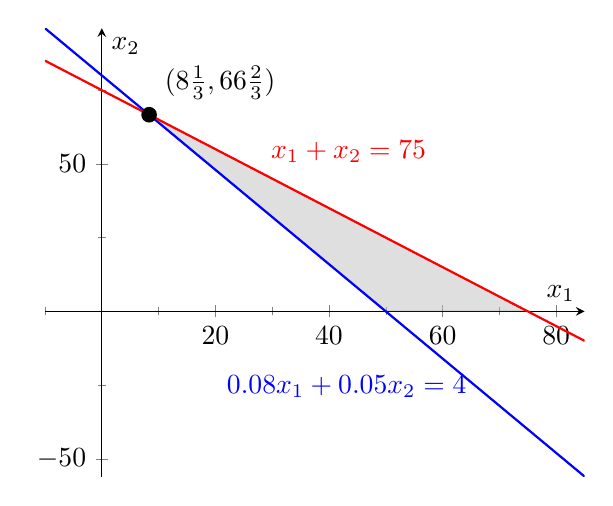
\begin{tikzpicture}
      \begin{axis}[
          axis lines=middle,
          xlabel=$x_1$,
          ylabel=$x_2$,
          minor tick num=1,
        ]
        \addplot[fill=gray!50, opacity=0.5] coordinates {(25/3,200/3) (50,0) (75,0)} -- cycle;
        \addplot[domain=-10:85, blue, thick] {(4-0.08*x)/0.05} node[left, pos=0.8] {$0.08x_1 + 0.05x_2 = 4$};
        \addplot[domain=-10:85, red, thick] {75-x} node[above right, pos=0.4] {$x_1 + x_2 = 75$};
        \node[fill=black, circle, inner sep=2pt, label={above right:$(8\frac13,66\frac23)$}] at (25/3,200/3) {};
      \end{axis}
    \end{tikzpicture}
  \end{center}
  Bound by convex region defined by axes, $x_1 + x_2 = 23$,
  and $0.08x_1 + 0.05x_2 = 4$ to give optimal solution at vertex
\end{sol}

\paragraph{Course overview}
\begin{itemize}[nosep]
  \item Formulation/modelling: create mathematical programs from problems
  \item Solving linear programs: use simplex method to optimize
  \item Geometric interpretation: conceptualize linear programs and simplex method
  \item Integer programs: linear programs defined over $\Z$
  \item Nonlinear programs: convex functions
\end{itemize}

\begin{defn}[optimization problem]
  Given a set of \term{feasible points} $A \subseteq \R^n$ and $f : A \to \R$,
  find some $x \in A$ that minimizes or maximizes the \term{objective value} $f(x)$.

  Composed of \term{decision variables} $\vb x \in \R^n$,
  the \term{objective function} $\max f(\vb x)$ or $\min f(\vb x)$,
  and some \term{constraints} of the form $g_i(\vb x) \leq b_i$
\end{defn}

\begin{defn}[affine function]
  Function of the form $f(\vb x) = \vb a^T \vb x + b = a_1x_1 + \dotsb + a_nx_n + b$ for constants $\vb a$ and $b$
\end{defn}

\begin{defn}[linear function]
  Affine function with $b=0$
\end{defn}

\begin{defn}[linear program]
  An optimization problem with affine objective function $f(\vb x)$ and finitely many linear constraint functions $g_i(x) \geq b_i$ (or $\leq b_i$ or $= b_i$) with constant $\vb b$.

  N.B.: constraints cannot be strict inequalities
\end{defn}

\section{LP Formulation}

\begin{example}
  A company makes 4 types of products, each requiring time on two different machines and two types of labour. The amount of machine time and labour needed to produce one unit of each product along with its sale price are summarized in the following table.
  \begin{center}
    \begin{tabular}{c|ccccc}
      Product & Machine 1 & Machine 2 & Skilled labour & Unskilled labour & Unit sale price \\ \hline
      1       & 11        & 4         & 8              & 7                & 300             \\
      2       & 7         & 6         & 5              & 8                & 260             \\
      3       & 6         & 5         & 5              & 7                & 220             \\
      4       & 5         & 4         & 6              & 4                & 180             \\
    \end{tabular}
  \end{center}
  Each month, the company can use up to 700 hours on machine 1, and 500 hours on machine 2, with no cost. The company can hire up to 600 hours of skilled labour at \$8 per hour, and up to 650 hours of unskilled labour at \$6 per hour. How should the company operate to maximize their monthly profit?
\end{example}
\begin{sol}
  Let $\vb x \in \R^4$ be number of units of products, $y_s$ and $y_u$ be hours of labour hired

  Let the objective function be $\max \enspace 300 x_1 + 260 x_2 + 220 x_3 + 180 x_4 - 8y_s - 6y_u$ (unit sale revenue net of labour costs)

  Let the constraints be $11x_1 + 7x_2 + 6x_3 + 5x_4 \leq 700$ (machine 1), $4x_1 + 6x_2 + 5x_3 + 4x_4 \leq 500$ (machine 2), $8x_1 + 5x_2 + 5x_3 + 6x_4 = y_s$, $7x_1 + 8x_2 + 7x_3 + 4x_4 = y_u$ (defining $y_s$ and $y_u$), $y_s \leq 600$, $y_u \leq 650$ (labour), and $x_1, x_2, x_3, x_4, y_s, y_u \geq 0$ (non-negativity)
\end{sol}

\lecture{May 4}
\begin{example}
  A certain company provides heading oil for the local commnity. They have historical data that helps them predict demand for heating oil in the next four months: 5000, 8000, 9000, 6000 (litres/month)

  At the beginning of each month, they can purchase oil from the supplier at the current market rate. The projected rates are given: 0.75, 0.72, 0.92, 0.90 (\$/litre)

  There is a storage tank that holds up to 4000 litres of oil, and at the start of month 1, it contains 2000 litres. How should the company buy the required oil to minimize the total money spent?
\end{example}
\begin{sol}
  Let $x_i$ be the amount of oil purchased in the $i$th month, and $y_i$ be the amount of oil in the storage tank at the start of month $i$.

  Then, we want to minimize $0.75x_1 + 0.72x_2 + 0.92x_3 + 0.9x_4$.

  The storage tank constrains us by $y_i \leq 4000$ and the problem gives $y_1 = 2000$.

  Non-negativity gives $x_i, y_i \geq 0$.

  For each demand $d_i$, we have $x_i + y_i = d_i + y_{i+1}$.

  Then, we can write:
  \begin{lp}{\min}{0.75x_1 + 0.72x_2 + 0.92x_3 + 0.9x_4}
     &  & y_1, y_2, y_3, y_4              & \leq 4000    \\
     &  & y_1                             & = 2000       \\
     &  & x_1 + y_1                       & = 5000 + y_2 \\
     &  & x_2 + y_2                       & = 8000 + y_3 \\
     &  & x_3 + y_3                       & = 9000 + y_4 \\
     &  & x_4 + y_4                       & = 6000       \\
     &  & x_1,x_2,x_3,x_4,y_1,y_2,y_3,y_4 & \geq 0
  \end{lp}
\end{sol}

\begin{example}
  Instead of minimizing the total money spent, suppose we do not have much money to spend each month, and we want to reduce the maximum amount spent in a month.
\end{example}
\begin{sol}
  Let $M = \max \{0.75x_1, 0.72x_2, 0.92x_3, 0.9x_4\}$.

  Since $M$ is not linear, we cannot simply put $\min M$ in an LP.

  Instead, define $m$ with constraints $m \geq 0.75x_1$, $m \geq 0.72x_2$, $m \geq 0.92x_3$, $m \geq 0.9x_4$.

  Since we are doing $\min m$, we are guaranteed that the optimal solution will give $m = M$ (if $m$ is not $M$, we can make $m$ smaller).
\end{sol}

\begin{example}
  Given a set of data points $\{(x_i, y_i) : i = 1,\dotsc,n\}$ on the plane. Find a line $y = ax + b$ that ``best fits'' this set of data points.
\end{example}
\begin{sol}
  Define ``best fit'' as minimizing total vertical distance between points and the line.

  That is, we must minimize $\sum \abs{ax_i + b - y_i}$, but that is not affine.

  Define instead the errors $e_i$ associated with the point $i$.

  We want to constrain $e_i = \abs{ax_i + b - y_i}$, which we can do with $e_i \geq ax_i + b - y_i$ and $e_i \geq y_i - ax_i - b$ since $\abs{x} = \max\{x, -x\}$.

  Then, we can use $\min \sum e_i$ as above to get the final LP:
  \begin{align*}
    \min \        & \sum e_i                \\
    \text{s.t.}\  & e_i \geq ax_i + b - y_i \\
                  & e_i \geq y_i - ax_i - b
  \end{align*}
  \textbf{N.B.:} since $e_i$, $e_j$ do not share constraints when $i \neq j$, $\min \sum e_i$ is equivalent to $\min e_1, \dotsc, \min e_n$.
\end{sol}

\begin{xca}
  Modify this to find the best fit parabola. Is this an LP?
\end{xca}
\begin{sol}
  Yes, since considering the error function $ax_i^2 + bx_i + c - y_i$ is still linear with respect to the variables for optimization $a$, $b$, and $c$.
\end{sol}

\section{Formulating IPs}

\lecture{May 9}
\begin{example}
  Consider the job application process where a company has 3 positions available, and there are 4 applicants for these jobs. For each applicant and position, the company assigns a number indicating how well the applicant is suited for the position. The goal is to hire a different applicant for each position to maximize the total suitability.

  \[
    M = \begin{pNiceMatrix}[first-row,first-col]
                                            & \Block{1-4}{\text{Candidates}} &   &   &   \\
      \Block{3-1}{\rotate \text{Positions}} & 3                              & 5 & 2 & 4 \\
                                            & 3                              & 1 & 4 & 3 \\
                                            & 1                              & 4 & 2 & 3
    \end{pNiceMatrix}
  \]
\end{example}
\begin{sol}
  Want: For each position, who gets that position

  Define: Create binary variable $x_{ij}$ for each position $i$ and candidates $j$. Let $x_{ij} = 1$ if position $i$ given to candidate $j$, and $0$ otherwise

  Objective function: $\max \sum\sum M_{ij}x_{ij}$

  Constraints: $\sum_{j} x_{ij} = 1$ for each $i$ (each position filled by exactly one candidate), and $\sum_i x_{ij} \leq 1$ for each $j$  (each candidate takes at most one position), $x_{ij} \geq 0$, $x_{ij} \leq 1$, $x_{ij} \in \Z$ (integrality)
  \begin{align*}\max\ & \sum_{i=0}^3\sum_{j=0}^4 M_{ij}x_{ij} \\ \text{s.t.}\ & \sum_{j=0}^4 x_{ij} = 1 & i = 1,\dotsc,3 \\ &\sum_{i=0}^3 x_{ij} \leq 1 & j = 1,\dotsc,4 \\ & 0 \leq x_{ij} \leq 1, x_{ij} \in \Z\end{align*}
\end{sol}

\begin{notation}
  We define $x \in \{0,1\}$ to mean the constraints $0 \leq x \leq 1$ and $x \in \Z$
\end{notation}

\begin{example}[Knapsack problem]
  There are 4 types of items that you can put into your backpack. You can take any integer number of units of any item. However, you can only carry a maximum of 40 pounds. Each unit of item you take is also worth a certain amount of money. The goal is to maximize the total value of the items you carry.
  \begin{center}
    \begin{tabular}{r|cccc}
      Item         & A  & B  & C  & D  \\ \hline
      Weight (lbs) & 1  & 7  & 3  & 2  \\
      Value (\$)   & 10 & 50 & 20 & 15 \\
    \end{tabular}
  \end{center}
\end{example}
\begin{sol}
  Let $x_i$, $i = A,B,C,D$ be the number of units of $i$ packed

  Objective function: $\max 10x_A + 50x_B + 20x_C + 15x_D$

  Constraints: $x_A + 7x_B + 3x_C + 2x_D \leq 40$ (weight limit), $x_i \geq 0$, $x_i \in \Z$ (integrality)

  \[
    \begin{aligned}
      \max\         &  & 10x_A + 50x_B + 20x_C + 15x_D           \\
      \text{s.t.}\  &  & x_A + 7x_B + 3x_C + 2x_D      & \leq 40 \\
                    &  & x_A,x_B,x_C,x_D               & \geq 0  \\
                    &  & x_A,x_B,x_C,x_D               & \in \Z
    \end{aligned}
  \]
\end{sol}

\begin{example}
  Suppose we are allowed to take A only if we take at least one unit of B.
\end{example}
\begin{sol}
  Want: if $x_B = 0$, then we must have $x_A = 0$. If $x_B \geq 1$, no restriction on $A$.

  Equivalently, add the constraint $x_A \leq x_B \max x_A = 40x_B$. When $x_B = 0$, the RHS goes to $0$ and constrains $x_A = 0$. Otherwise, since $x_B \geq 1$, $40x_B \geq 40$ which is the maximum value of $x_A$, so there are effectively no constraints on $x_A$.
\end{sol}

\begin{example}
  Suppose we want the following conditions to hold:
  \begin{enumerate}[1.,nosep]
    \item We carry at least 5 units of items A and/or B; or
    \item We carry at least 7 units of items C and/or D.
  \end{enumerate}
\end{example}
\begin{sol}
  Define a binary variable $y$. Want: $y = \begin{cases*}1&condition 1 is true\\0&condition 2 is true\end{cases*}$

  If $y = 1$, then $x_A + x_B \geq 5$; if $y = 0$, no restrictions on $x_A$, $x_B$. We can implement this by adding the constraint $x_A + x_B \geq 5y$, since $y = 0$ will send the RHS to $0$

  If $y = 0$, then $x_C + x_D \geq 7$; if $y = 1$, no restrictions on $x_C$, $x_D$. Similarly implement with $x_C + x_D \geq 7(1-y)$, since $y=1$ will send the RHS to $0$

  Notice that setting $y$ does not force the other condition \emph{not} to hold, i.e., this implements an inclusive or.

  In summary: $x_A + x_B \geq 5y$, $x_C + x_D \geq 7(1-y)$, and $y \in \{0,1\}$

  \textbf{N.B.:} When feeding these constraints into an algorithm, ensure that the constraints are truly linear, i.e., move variables to one side. For example, $x_A + x_B - 5y \geq 0$
\end{sol}

\begin{xca}
  Implement an exclusive or of these two conditions
\end{xca}

\begin{example}
  Suppose that the value of item A is \$10 for the first 5 units, but any more units beyond that has value \$5.
\end{example}
\begin{sol}
  Separate $x_A$ into two variables $x_{A1}$ for first five units and $x_{A2}$ for remainder.
  Then, we have $x_A=x_{A1}+x_{A2}$ and change the objective function to $10x_{A1} + 5x_{A2} + 50x_B + 20x_C + 15x_C$.

  We can create a constraint to force $x_{A2}$ only to go up when $x_{A1}$ is 5 with $x_{A2} \leq (x_{A1} - 4)\max x_{A2}$ which will work in tandem with the non-negativity constraint. This is not actually necessary since the maximum will always fill $x_{A1}$ before $x_{A2}$ because it is worth more (i.e. trading one $x_{A2}$ for $x_{A1}$ will increase the objective function by 5)

  In summary: change the objective function and add the constraints $x_A = x_{A1} + x_{A2}$, $x_{A1} \leq 5$, $x_{A1},x_{A2} \geq 0$, $x_{A1}, x_{A2} \in \Z$
\end{sol}

\lecture{May 11}
\begin{notation}[vector notation]
  Write $\mathbb{1} := (1,\dotsc,1)^T$ and $x \leq y$ if $x_i \leq y_i$ for all $i$.
\end{notation}

\begin{defn}[graph]
  $G = (V, E)$ consists of a set of objects $V$ (\term{vertices}) and a set of unordered pairs of vertices $E$ (\term{edges}).

  We restrict graphs by disallowing empty graphs, redundant edges, directed edges, or self-connections.
\end{defn}

\begin{example}\label{ex:graph}
  $G = (V, E)$ by $V = \{1,2,3,4\}$, $E=\{12,23,34,41,24\}$
  \begin{center}
    \tikz\graph{{1,4}--{2,3}; 1--4; 2--3; 2--4};
  \end{center}
\end{example}

\begin{defn}[incidence relation]
  For an edge $e=uv$, $e$ is incident to $u$ and $v$.
  $\delta(v)$ is the set of all edges incident to $v$.

  The \term{incidence matrix} $B \in \{0,1\}^{\abs{V}\times\abs{E}}$
  has rows indexed by $V$, columns by $E$, and $B_{ve} = 1$
  when $e \in \delta(v)$ and $0$ otherwise.
\end{defn}
\begin{example}
  For \cref{ex:graph}, $B = \begin{pNiceMatrix}[first-row,first-col]
        & e_1 & e_2 & e_3 & e_4 & e_5 \\
      1 & 1   & 0   & 0   & 1   & 0   \\
      2 & 1   & 1   & 0   & 0   & 1   \\
      3 & 0   & 1   & 1   & 0   & 0   \\
      4 & 0   & 0   & 1   & 1   & 1
    \end{pNiceMatrix}$.
\end{example}
\begin{remark}
  Each column has exactly two ones, so $B\mathbb{1} = 2\mathbb{1}$.
\end{remark}

\begin{defn}[matching]
  $M \subseteq E$ where each vertex is incident with exactly zero or one edge in $M$ (i.e., $\abs{M \cap \delta(v)} \leq 1$ for all $v \in V$)
\end{defn}
\begin{example}
  For \cref{ex:graph}, $\{e_1, e_3\}$ and $\{e_5\}$ are matchings but $\{e_1, e_5\}$ is not since $2$ is incident to both edges
\end{example}

\begin{example}[maximum-weight matching]
  Given graph $G = (V, E)$ and weights $w_e$ for each $e \in E$. Find a matching in $G$ with the maximum edge weight, i.e., maximize $\sum_{e \in M} w_e$.
\end{example}
\begin{sol}
  Define a vector $x \in \{0,1\}^{\abs{E}}$ by $x_e = 1$ if $e \in M$ and $0$ otherwise.
  Then, the objective function is $\max w^T x$.
  To ensure each node appears only once, add constraints $\sum_{e \in \delta(v)} x_e \leq 1$ for each $v \in V$. This is equivalent to taking the incidence matrix $A$ and saying $Ax \leq \mathbb{1}$
  This gives us the integer program
  \begin{align*}
    \max\         & w^T x                         \\
    \text{s.t.}\  & Ax \leq \mathbb{1}            \\
                  & x_e \in \{0,1\} \quad e \in E
  \end{align*}
\end{sol}

\begin{defn}[$v_1$,$v_k$-path]
  Sequence of edges $v_1v_2, v_2v_3, \dotsc, v_{k-1}v_k$ such that $v_1,\dotsc,v_k$ are distinct
\end{defn}
\begin{example}\label{ex:path}
  Consider graph $(\{s,t,a,b,c,d\}, \{sa,sc,ab,ac,bd,bt,cb,cd,dt\})$.
  \begin{center}
    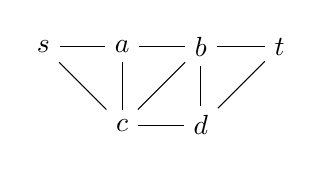
\begin{tikzpicture}
      \graph[math nodes]{s--{a--b,c--d}--t; a--c; b--d; c--b};
    \end{tikzpicture}
  \end{center}  
  Then, $sa,ab,bt$ and $sc,cb,bd,dt$ are $s$,$t$-paths but $sa,ab,bc,cd,cb,bt$ is not since $b$ is visited twice.
\end{example}

\lecture{May 16}

\begin{problem}[shortest path]
  Given graph $G = (V, E)$, vertices $s$ and $t$, and positive weights $w_e$ for each $e \in E$. Find an $s$,$t$-path $P$ with the minimum edge weight, i.e., minimize $\sum_{e \in P} w_e$.
\end{problem}

Define a vector $x \in \{0,1\}^{\abs{E}}$ by $x_e = 1$ if $e \in P$ and $0$ otherwise.

The objective function is $\min w^T x$.

Need to constrain $x$ into a path: use cuts.

\begin{defn}[cut]
  The \term*{cut induced by vertices $W$} is the set $\delta(W)$ of all edges with exactly one endpoint in $W$.
  Formally, $\delta(W) = \{uv \in E : u \in W, v \not\in W\}$.

  An \term{$s,t$-cut} $\delta(W)$ has $s \in W$ and $t \not\in W$.
\end{defn}
\begin{example}
  In \cref{ex:path}, $W=\{s,a,b\}$ induces the cut $\delta(W) = \{sc,ac,bc,bd,bt\}$
  \begin{center}
    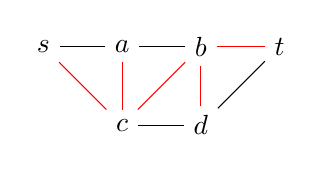
\begin{tikzpicture}
      \graph[math nodes,simple]{s--{a--b,c--d}--t; s--[red]c; a--[red]c; b--[red]d; b--[red]c; b--[red]t};
    \end{tikzpicture}
  \end{center}
\end{example}

\begin{prop}
  Notice that the edges in an $s,t$-cut separate $s$ from $t$, so an $s,t$-path must use at least one edge from every $s,t$-cut (formal proof in graph theory course)
\end{prop}

We get a constraint $\sum_{e \in \delta(W)} x_e \geq 1$ for all $s,t$-cuts $\delta(W)$ (that is, for all $W \subset V$ with $s \in W$ and $t\not\in W$)

\begin{prop}
  If a set of edges intersects every $s,t$-cut, then it contains an $s,t$-path
\end{prop}

Minimizing the edge weights will ensure that the extraneous edges are optimized away and the $s,t$-path remains so long as the edge weights are all positive.

This gives us a final IP of
\begin{align*}
  \min\         & w^T x                                                               \\
  \text{s.t.}\  & \sum_{e \in \delta(W)} x_e \geq 1 & \text{$\delta(W)$ an $s,t$-cut} \\
                & x_e \geq 0, x_e \in \Z            & e \in E
\end{align*}

\section{Formulating NLPs}

\begin{defn}[non-linear program]
  A program of the general form $\min f(x)$ subject to $g_i(x) \leq 0$ for some arbitrary functions $f : \R^n \to \R$, $g_i : \R^n \to \R$ with no restrictions
\end{defn}
\begin{example}
  Among all the points $x$ that satisfy $Ax \leq b$, find one that is closest to the target point $\bar x$
\end{example}
\begin{sol}
  We can take the norm and minimize $\norm{x - \bar x} = \sqrt{\sum(x_i-\bar x_i)^2}$.
  This gives us the non-linear program $\min \norm{x - \bar x}, \text{s.t.\ } Ax \leq b$.
\end{sol}

\lecture{May 18}
Since the definition for NLP has no constraints on $f$ and $g_i$, a LP is an NLP.

The integrality constraint makes IPs not NLPs.
To get around this, use a periodic function like $\sin \theta = 0$ which permits values $\theta = k\pi$ for integer $k$, so $x \in \Z \Harr \sin x\pi  = 0$.
Using this makes IPs into NLPs.

If we can solve NLPs, we can also solve LPs and IPs.

\section{LP outcomes}

An algorithm that solves LPs should produce:
\begin{itemize}[nosep]
  \item The optimal solution (or that no solution exists)
  \item Certificate of correctness that reduces complexity of verification
\end{itemize}

\begin{defn}[infeasibility]
  No feasible solutions exist.
\end{defn}

\begin{example}
  $\max x$ s.t. $x \leq 2$ and $x \geq 3$. Obviously, no $x$ exists.
\end{example}

\begin{example}
  $\max{(3,1,-7,4)x}$ s.t. $\mqty(-5&4&3&-1\\2&1&-5&3\\-1&-3&1&-2)x = \mqty(3\\-2\\1)$ and $x \geq \mathbb{0}$.

  Taking $-2R_1 - 3R_2 - 4R_3$, we get $8x_1+x_2+5x_3+x_4 = -4$ but each entry in $x$ must be non-negative, so this is impossible.

  Formally, we can let $y = (-2,-3,-4)^T$, then multiply on the left by $y^T$ to give us the same equation as $(8,1,5,1)x = -4$.

  Then, $y$ is the \term{certificate of infeasibility}.
\end{example}

\begin{prop}
  The system $Ax = b$, $x \geq \mathbb{0}$ is infeasible if there exists a vector $y$ such that $y^T A \geq \mathbb{0}$ but $y^T b < 0$
\end{prop}
\begin{prf}
  Suppose the system is feasible with $x$ as the feasible solution. Then, $Ax = b$ and $x \geq \mathbb{0}$. However, $y^T A x \geq 0$ and $y^T b < 0$. Contradiction.
\end{prf}

The converse is also true. Proof will come later as Farkas' Lemma.

\begin{defn}[unboundedness]
  Infinitely better feasible solutions exist.

  Formally, a max (resp. min) LP is \term*{unbounded} if there exists a series of feasible solutions $x(t)$ with the objective value of $x(t)$ approaching $+\infty$ (resp. $-\infty$) as $t \to \infty$.
\end{defn}
\begin{example}
  $\max x$ s.t. $x \geq 1$: there is no best solution (cf. strict inequalities)
\end{example}
\begin{example}
  $\max{} (-1,2,-3,4)x$ s.t. $\mqty(3&0&2&-5\\-2&3&-4&4)x=\mqty(4\\1)$ and $x \geq \mathbb 0$.

  Consider $\bar x = (3,1,0,1)^T$ and $d = (0,4,5,2)^T$. Define $x(t) = \bar x + td$ and consider $t$ from $0 \to \infty$.
  We must show feasibility and unboundedness.

  Obviously, $x(t) \geq \mathbb 0$ since $\bar x, d \geq \mathbb 0$ and $t \geq 0$.

  Notice $Ax(t) = A\bar x + tAd = (4,1)^T + t(0,0)^T = b$. That is, $\bar x$ solves $Ax = b$ and $d$ lies in the kernel of $A$.

  The objective value $c^T x(t) = c^T(\bar x + td) = c^T\bar x + tc^T d = 3 + t$ clearly goes to $+\infty$ as $t \to \infty$.

  Then, $(\bar x, d)$ is a certificate of unboundedness for the LP.
\end{example}

\begin{prop}
  The LP $\max \{c^T x : Ax=b, x \geq \mathbb 0\}$ is unbounded if there exist vectors $\bar x$ and $d$ such that $\bar x, d \geq \mathbb 0$, $Ad = \mathbb 0$, $c^T d > 0$.
\end{prop}


\chapter{Solving LPs}
\section{Preparation}
\lecture{May 23}

\begin{example}
  $\max{} (0,-2,-3,0)x+7$ subject to $\mqty(1&3&-5&0\\0&-1&2&1)x=\mqty(6\\9)$ and $x \geq \mathbb 0$
\end{example}

\begin{sol}
  Trivial solution: $\bar x = (6,0,0,9)\trans$ gives objective value 7

  Claim: $\bar x$ is optimal

  Proof: the term $(0,-2,-3,0)x \leq 0$ since $x \geq \mathbb 0$.
  Its highest value is then 0, so the highest objective value is 7.
  Since the objective value of $\bar x$ is 7, it is optimal.
\end{sol}

\begin{theorem}[Fundamental Theorem of Linear Programming]
  For a linear program $P$, exactly one of the following holds:
  \begin{itemize}[nosep]
    \item $P$ is infeasible
    \item $P$ is unbounded
    \item $P$ has an optimal solution
  \end{itemize}
\end{theorem}

This does not apply to non-linear programs: e.g., $\max x$ subject
to $x < 1$. This NLP is feasible (consider $\bar x = 0$) and
bounded ($x < 1$), but has no optimal solution (given $\bar x$ a
solution, $\frac{\bar x+1}{2}$ is a better solution)

\begin{defn}[standard equality form]
  A linear program of the form
  $\max \{c\trans x + \bar z : Ax = b, x \geq \mathbb 0\}$

  Requires maximization, equality constraint, and non-negative
  variables
\end{defn}

Simplex requires SEF, so must convert LPs into equivalent SEF LP.

\begin{defn}[equivalence]
  $P$ and $P'$ are equivalent if
  (1) $P$ infeasible iff $P'$ infeasible,
  (2) $P$ unbounded iff $P'$ unbounded, and
  (3) optimal solutions of $P$ can be constructed from $P'$ and vice versa
\end{defn}

Find an equivalent SEF by:

\begin{itemize}[nosep]
  \item Given a minimization LP $\min f(x)$, just take $\max -f(x)$
  \item Given an inequality $x \leq k$, define a slack variable
        $x + x' = k$ with $x' \geq 0$
  \item Given a free variable $x$, define two non-negative variables
        $x^+$ and $x^-$ so that we can replace $x = x^+ - x^-$
\end{itemize}


\begin{example}
  Find an equivalent LP in SEF
  \begin{align*}
    \min         & (-1,2,-3)x             \\
    \text{s.t. } & \mqty(1        & 5 & 3 \\2&-1&2\\1&2&-1)\mqty(x_1\\x_2\\x_3)\mqty{\leq\\\geq\\=}\mqty(5\\4\\2) \\
                 & x_1,x_2 \geq 0
  \end{align*}
\end{example}
\begin{sol}
  Switch $\min$ to $\max$ with new objective function $(1,-2,3)x$

  Divide $x_3 = x_3^+ - x_3^-$ giving $\mqty(1&5&3&-3\\2&-1&2&-2\\1&2&-1&1)\mqty(x_1\\x_2\\x_3^+\\x_3^-)$

  Add slack variables $x_4$, $x_5$ giving new rows $(1,5,3,1,0)x=5$
  and $(2,-1,2,0,1)x=4$

  Let $x = (x_1,x_2,x_3^+,x_3^-,x_4,x_5)\trans$
  and combine to get the SEF
  \[\max \qty{ (1,-2,3,-3,0,0)x : \mqty(1&5&3&-3&1&0\\2&-1&2&-2&0&1\\1&2&-1&1&0&0)x=\mqty(5\\4\\2), x \geq \mathbb 0}\]
  Suppose simplex solves this and gives optimal solution
  $(\frac{11}{4},0,\frac34,0,0,3)\trans$ with optimal value $5$. Then, the
  original LP is solved by
  $(\frac{11}{4},0,\frac34-0)\trans =(\frac{11}{4},0,\frac34)$ with optimal
  value $-5$.
\end{sol}

\lecture{May 25}
\begin{example}
  $\max (3,-2,0,0,0)x$ such that $x \geq \mathbb 0$
  and $\mqty(4&-1&1&0&0\\3&-3&0&1&0\\-2&2&0&0&1)x=\mqty(8\\9\\1)$
\end{example}
\begin{sol}
  Feasible solution: $\bar x = (0,0,8,9,1)\trans$ with objective value
  $(3,-2,0,0,0)(0,0,8,9,1)\trans = 0$

  To increase objective value, must increase $x_1$ (the only one
  with a positive coefficient in the objective function)

  Change $x_1 \mapsto t$, keep $x_2 = 0$, and set
  $x_3 \mapsto 8-4t$, $x_4 \mapsto 9-3t$, and $x_5 \mapsto 1+2t$
  to maintain feasibility

  But we still have non-negativity, giving us $t \leq 2$, i.e.,
  $\bar{\bar x} = (2,0,0,3,5)\trans$
\end{sol}

This example worked because we had (1) the identity matrix embedded
in columns, (2) those columns have zero coefficients in the
objective function.
Equivalent strategies will exist if the matrix's rows are
independent.

\begin{notation}
  Given a matrix $A$, notate the column $j = 1,\dotsc,n$ of $A$ by
  $A_j$ and then the submatrix formed by columns
  $J \subseteq \{1,\dotsc,n\}$ by $A_J$
\end{notation}

\begin{prop}
  \Tfae: $B \subseteq \{1,\dotsc,n\}$ is a basis;
  $A_B$ is invertible; and
  $\abs{B} = m$ and the columns $A_B$ are linearly independent
\end{prop}

\begin{defn}
  Given a basis $B$, a \term{non-basis}
  $N = \{1,\dotsc,n\}\setminus B$.

  The variables $x_B$ where $B$ a basis are \term{basic variables};
  conversely, $x_N$ are \term{non-basic variables}.
  This lets us write $Ax = A_Bx_B + A_Nx_N$.

  A \term{basic solution} (with respect to $B$) is a solution $x$ where $x_N = 0$.
\end{defn}

To find a basic solution $x_B$, multiply both sides of the
constraint $Ax = b$ on the left by $A_B^{-1}$. Then,
$A_B^{-1}Ax = A_B^{-1}b$ and we can read the basic solution
$x_B = A_B^{-1}b$.

\begin{defn}[basic feasible solution]
  A value $\bar x$ such that $\bar x_B \geq \zero$.
\end{defn}

\begin{defn}[canonical form]
  SEF $\max\{c\trans x+\bar z:Ax=b,x\geq\mathbb0\}$ if $A_B=I$ and
  $c_B=\mathbb 0$
\end{defn}

\lecture{May 30}

\begin{example}
  Write the canonical form for $B=\{2,3\}$ of
  $\max (3,-1,4,0,-1)x + 2$ s.t. $x \geq \mathbb 0$ and
  $\mqty(2&1&-2&5&-4\\-1&0&-1&-3&2)x = \mqty(3\\-2)$
\end{example}

\begin{sol}
  Multiply the constraint on the left by
  $A_B^{-1} = \mqty(1&-2\\0&-1)$ to get new constraint
  $\mqty(4&1&0&11&-8\\1&0&1&3&-2)x=\mqty(7\\2)$ which is equivalent

  Then, we need to set the entries in the objective function vector
  $c_B = \mathbb 0$

  To find an expression for $-c_B\trans x_B$ which can cancel, take
  $-c_B\trans Ax = -c_B b$ to get
  $(0,1,-4,-1,0)x = -1 \implies (0,1,-4,-1,0)x + 1 = 0$

  Add this to $c\trans x + \bar z$ to get the new objective function
  $\max (3,0,0,-1,-1)x + 3$
\end{sol}

In general, to convert from SEF to canonical form given a basis $B$:

\begin{enumerate}[1.,nosep]
  \item Amend the constraint: $Ax = b \mapsto A_B^{-1} A x = A_B^{-1} b$
  \item Calculate $y = (A_B^{-1})\trans c_B$
        (this will be used later as a certificate)
  \item Amend the objective function:
        $c\trans x + \bar z \mapsto (c\trans - y\trans A)x + (\bar z - y\trans b)$
\end{enumerate}

\section{Simplex}

Main idea: go between feasible bases, attempting to raise the objective value
\begin{enumerate}
  \item Start with a feasible basis $B$.

        Use ``2-phase simplex'' to find one if there is not a trivial feasible basis
  \item Convert the LP to canonical form with respect to $B$.

        If $c_N \leq \mathbb 0$, then the optimal solution is the basic
        feasible solution. \textbf{Stop}.
  \item Pick a non-basic entering variable $x_k$ where $c_k > 0$.

        (Bland's rule) Pick the variable with lowest index $k$.

        If $A_k \leq \mathbb 0$, then the linear program is
        unbounded. \textbf{Stop}.

        Increase $x_k = t$ while reducing $x_B$
        to increase the objective value, i.e., maximize $t$ subject to
        $x_B = b - A_k t$ and $x \geq \mathbb 0$.
        That is,
        $t = \min\{\frac{b_i}{A_{ik}} : A_{ik} > 0\}$
  \item Pick a leaving variable $x_\ell$.

        Let $x_\ell$ be the index used for the minimum
        above. Then, $x_\ell = 0$ after setting $x_k = t$ making $x_\ell$
        non-basic.

        Repeat step 2 with the new basis
        $B = B \cup \{k\} \setminus\{\ell\}$
\end{enumerate}

\begin{example}
  Maximize $(0,2,1,0,0,0)x$ such that
  $x \geq \mathbb 0$ and
  \[\mqty(\mqty{1&-1&1\\-2&1&0\\0&1&-2}&\mqty{\imat{3}})x = \mqty(5\\3\\5)\]
\end{example}
\begin{sol}
  Perform simplex:
  \begin{enumerate}
    \item Entering variable $x_2$ since $c_2 = 2 > 0$

          Set $x_2 = t = \min\{-,\frac{3}{1},\frac{5}{1}\} = 3$

          Leaving variable is $x_5$, new basis $B = \{2,4,6\}$

          New canonical form $\max(4,0,1,0,-2,0)x + 6$ with
          $x \geq \mathbb 0$ and
          \[\mqty(-2&1&0&0&1&0\\-1&0&1&1&1&0\\2&0&2&0&-1&1)x = \mqty(3\\8\\2)\]

    \item Entering variable $x_1$.
          Set $x_1 = t = \min\{-,-,\frac{2}{2}\}=1$.

          Leaving variable $x_6$. New basis $B = \{1,2,4\}$

          New canonical form $\max(0,0,5,0,0,-2)x + 10$ with
          $x \geq \mathbb 0$ and
          \[\mqty(1&0&-1&0&-\frac12&\frac12\\0&1&-2&0&0&1\\0&0&0&1&\frac12&\frac12)x = \mqty(1\\5\\9)\]

    \item Entering variable $x_3$.
          Set $x_3 = t = \min\{-,-,-\} = \infty$.
          No bound on $t$, so this LP is unbounded.
  \end{enumerate}
  \lecture{June 1}
  Iteration 3 entered $x_3$, and $A_3 \leq 0$.
  Then, $t$ had no bounds, so the LP is unbounded.
  Find a certificate of unboundedness:

  Current basic feasible solution: $\bar x = (1,5,0,9,0,0)\trans$

  Set $x_3 = t$.
  New solution is $x(t) = (1+t,5+2t,t,9,0,0)\trans = \bar x + td$
  where $d = (1,2,1,0,0,0)\trans$.

  Then, $x(t)$ is feasible for all $t \geq 0$ and
  $c\trans x(t) = 5t - 10 \to \infty$.
  This is all we need to show that $(\bar x, t)$
  form a certificate of unboundedness.
\end{sol}


Recall: simplex iterates over feasible bases to optimize one variable
at a time and set coefficients to zero, eventually finding an optimal
solution or showing unboundedness

Does simplex always terminate? Intuitively it should, since each
iteration increases the objective value. However, this is not true in
general

\begin{defn}[degenerate iteration]
  Iteration where the objective value is held constant.
  That is, only the basis is changed.
\end{defn}

\begin{example}
  Maximize $(1,0,0,0)x$ subject to $x \geq \mathbb0$
  and $\mqty(3&2&1&0\\1&1&0&1)x = (0,2)\trans$.

  The start basis is clearly $\{1,4\}$
  The only entering variable is $x_1$. Let $t = x_1$ and
  $t = \min\{\frac21,\frac03\} = 0$
  We pick $x_4$ for a leaving variable, giving $B' = \{1,4\}$,
  which is the same.
\end{example}

\begin{defn}[cycling]
  Repeating bases with the same basic feasible solution.
\end{defn}

This happens when there is a series of degenerate iterations that repeat bases already used.
Bland's Rule, when applied, prevents cycling and guarantees simplex terminates.
That is, when there is a choice for the entering or leaving variable,
pick the one with the lowest index.

\paragraph{\term{Tableau method} \rm (easier to perform by hand)}
Use a matrix to encode the entire state of the algorithm, allowing
row reductions to replace taking inverses

\begin{example}
  Maximize $z = (3,-2,0,0,0)x+0$ subject to
  $x \geq \mathbb0$ and
  \[\mqty(\mqty{4&-1\\3&-3\\-2&2}&\mqty{\imat{3}})x = \mqty(8\\9\\1)\]
\end{example}
\begin{sol}
  Create a tableau
  $\qty(\begin{array}{c|c|c}1 & -c& \bar z \\ \hline \mathbb0 & A & B\end{array}) = \qty(\begin{array}{c|ccccc|c}1&-3&2&0&0&0&0 \\\hline 0&4&-1&1&0&0&8 \\ 0&3&-3&0&1&0&9 \\ 0&-2&2&0&0&1&1 \end{array})$

  Entering variable: look for negative coefficient in objective row
  $x_k$ (in this case $x_1$)

  Leaving variable: look at ratio between $b$ and $A_k$ to find
  row with $x_\ell$ (in this case $A^1$)

  Take the entry in column of $x_k$ and the row of $x_\ell$
  (in this case $A_{11}$).
  Use row operations to make it 1 and the rest of the column 0.

  In this case $\frac14R_2$, $R_1 + 3R_2$, $R_3 - 3R_2$,
  $R_4 + 2R_2$, to yield
  $\qty(\begin{array}{c|ccccc|c}1&0&\frac54&\frac34&0&0&6 \\\hline 0&1&-\frac14&\frac14&0&0&2 \\ 0&0&-\frac94&-\frac34&1&0&3 \\ 0&0&\frac32&\frac12&0&1&5 \end{array})$

  Since top row is all positive, this means that $c$ is all
  negative, so we have an optimal solution with optimal
  objective value 6
\end{sol}

Since tableau method involves iterative dividing of decimals,
computers will lose precision after each iteration. With canonical
form, calculations are always done from the original LP, so no
compounded error.

If no obvious basic feasible solution to start simplex, do two-stage
simplex.

\section{Two-phase simplex}

Main idea: Form an auxiliary LP with an obvious BFS, then solve with simplex to
help find a BFS or prove that no BFS exists
\begin{itemize}[nosep]
  \item Negate constraints with negative right-hand sides
  \item Arbitrarily add auxiliary variables to append an identity matrix
        to $A$
  \item Apply simplex to the new LP: there is a solution to the original
        LP if and only if this LP has solutions with the auxiliary
        variables set to zero
\end{itemize}

\begin{example}
  Maximize $(-3,2,0,0,0)x$ subject to
  $x \geq \mathbb0$ and
  \[\mqty(\mqty{-1&1\\-1&-2\\0&1}&\mqty{\imat{3}})x = \mqty(-1\\-4\\4)\]
\end{example}
\begin{sol}
  Notice that $B = \{3,4,5\}$ is a basis.
  However, the trivial basic solution $(0,0,-1,-4,4)\trans$ is not feasible.

  Negate constraints to get
  $\mqty(\mqty{1&-1&-1&0&0\\1&2&0&-1&0\\0&1&0&0&1})x = \mqty(1\\4\\4)$.

  Add auxiliary variables to get
  $\mqty(\mqty{1&-1&-1&0&0\\1&2&0&-1&0\\0&1&0&0&1}&\mqty{\imat{3}})x = \mqty(1\\4\\4)$.

  This LP has a BFS $(0,0,0,0,0,1,4,4)\trans$.

  \lecture{June 6}
  Start with $B = \{6,7,8\}$ with BFS
  $\bar x = (0,0,0,0,0,1,4,4)\trans$.

  Minimize the sum of auxiliary variables:
  $\min{(0,0,0,0,0,1,1,1)x}$ subject to same constraints.

  Same as saying $\max{(0,0,0,0,0,-1,-1,-1)x}$, which we can solve
  with simplex.

  If optimal value is 0, then auxiliary variables must be 0.
  If optimal value is negative, no feasible solution exists.

  Based on canonical form, multiply constraint on left by $(1,1,1)$
  to get $(2,1,-1,-1,1,1,1,1)x-9=0$.

  Add to objective function to get new objective function
  $(2,1,-1,-1,1,0,0,0)x-9$.

  Run simplex to get basis $\{1,3,5\}$ and BFS
  $(4,0,3,0,4,0,0,0)\trans$.

  Now that we have a BFS $(4,0,3,0,4)\trans$, run simplex.
\end{sol}

If auxiliary LP does not have a solution, then $y = A_B^{-T}x_B$ is
a certificate of infeasibility for the original LP.

Optimal solution must exist: it is feasible by construction and not
unbounded because the objective value cannot exceed 0.

Therefore, two-phase simplex will always work.

\section{Geometry of simplex}
Consider $\max{(1,1)x}$ subject to
$x \geq \mathbb0$ and $\mqty(1&0\\0&1\\2&1)x \leq \mqty(4\\3\\4)$.

Equivalently, $\max{(1,1,0,0,0)x}$ subject to $x \geq \mathbb0$ and
$\mqty(\mqty{\imat2\\2&1}&\mqty{\imat3})x = \mqty(4\\3\\4)$.

Equalities define lines, inequalities define halfspaces:
\lecture{June 8}
\begin{itemize}[noitemsep]
  \item Non-negativity bounds $(x_1, x_2) \in \R^2$ to the first quadrant.
  \item Constraints bound $x_1 \leq 4$, $x_2 \leq 3$, and $x_1 + 2x_2 \leq 8$.
\end{itemize}
All feasible solutions are thus contained in the convex polygon bounded by
$(0,0)$, $(0,3)$, $(2,3)$, $(4,2)$, $(4,0)$.

Consider contours of the objective function $x_1 + x_2 = k$ starting at $k=0$.
Imagine dragging the objective function line ``up'' along the normal
vector $(1,1)\trans$ maintaining the slope.
Last point $(4,2)\trans$ which touches the highest contour $k=6$ is
the optimal solution.

Notice that $(4,2)\trans$ is generated by $x_1=4$ and $x_1 + 2x_2 = 8$,
i.e., setting constraints (1) and (3) to equality.
Then, in SEF, $(4,2)\trans \mapsto (4,2,0,1,0)\trans$ is a BFS.

Likewise, consider the extreme point $(4,0)\trans$
generated by $x_1 = 4$ and $x_2 = 0$, i.e.,
constraints (1) and (5) to equality.
In SEF, $(4,0)\trans \mapsto (4,0,0,3,4)\trans$ which is a BFS.

We can make some observations.

\begin{defn}[boundary]
  A point $p \in S$ is on the \term*{boundary of $S$}
  if every open neighbourhood of $p$
  contains a point in $S$ and a point not in $S$.
\end{defn}

\begin{remark}
  Optimal solutions must always be on the boundary.
\end{remark}

\begin{defn}[tight constraint]
  An inequality satisfied with equality by a feasible solution $\bar x$.
\end{defn}

\begin{theorem}
  If an optimal solution exists and the rows of $A$ are linearly independent,
  then there is at least one optimal ``corner''.
\end{theorem}
\begin{prf}
  Setting inequality to equality means setting a slack variable in SEF to 0.
  Every corner point is defined by $n$ linear equalities in $\R^n$,
  i.e., $n$ (or more) tight constraints.
  Therefore, a corner point's canonical form solution will have
  $n$ slack variables set to zero, creating a BFS.
\end{prf}

Geometrically, simplex walks along extreme points (BFSs) until it finds an optimal solution.
Two-phase simplex is required when the origin is not available as a corner to start from.
Each iteration picks an adjacent extreme point,
because it swaps one tight constraint for another one and maintains the other $n-1$ constraints.

\begin{defn}[degenerate]
  $\bar x$ with more than $n$ tight constraints, i.e., some basic variables are 0.
\end{defn}

This means an iteration may bounce endlessly between degenerate BFSs.
Degenerate iterations are avoided by Bland's rule.

Finally, simplex requires that the feasible region be convex.
It always is because it is the convex hull generated by the extreme points.

\lecture{June 13}

Formalize some basic geometric ideas from last lecture.

\begin{defn*}[geometry]
  A \term{hyperplane} is an equation of the form $a\trans x = \beta$ with
  \term{normal vector} $a$.

  A \term{halfspace} is an inequality of the form $a\trans x \leq \beta$
  with \term*{normal vector} $a$. Note: the halfspace is always on the
  opposite side of the normal vector.

  A \term{polyhedron} is a set of points
  $\{x \in \R^n : Ax \leq b\}$, i.e., the intersection of $m$
  halfspaces for a polytope with $m$ facets.
\end{defn*}

\begin{defn}[convexity]
  Subset $S \subseteq \R^n$ such that for all
  $x^1, x^2 \in S$ and $\lambda \in [0,1]$,
  $\lambda x^1 + (1-\lambda)x^2 \in S$.
  This expression is a \term{convex combination}.
\end{defn}

\begin{prop}
  A halfspce is convex.
\end{prop}
\begin{prf}
  Let $H = \{x \in \R^n : a\trans x \leq \beta\}$ be a halfspace and $x^1, x^2 \in H$.
  Then, with arbitrary $\lambda \in [0,1]$, let $x = \lambda x^1 + (1-\lambda)x^2$.

  We have $a\trans x = \lambda a\trans x^1 + (1-\lambda) a\trans x^2$.
  But since $x^1, x^2 \in H$, we get
  $a\trans x \leq \lambda \beta + (1-\lambda)\beta = \beta$ as desired.
\end{prf}

\begin{prop}
  The intersection of convex sets is convex.
\end{prop}
\begin{prf}
  If two points are in the intersection, they are in each convex set.
  The line segment joining them is then also in each convex set,
  meaning it is in the intersection.
\end{prf}

\begin{corollary}
  A polyhedron is convex.
\end{corollary}

\begin{defn}[extreme point]
  Point $\bar x \in C$ a convex set such that $x$ is not
  a convex combination of two distinct points in $C$ distinct from $\bar x$.
\end{defn}

\lecture{June 15}

\begin{theorem}[characterization of extreme points in polyhedra]\label{thm:xp-r}
  For $\bar x \in P = \{x \in \R^n : Ax \leq b\}$ a polyhedron
  where $A^=x = b^=$ is the set of tight constraints for $\bar x$,
  $\bar x$ is an extreme point of $P$ if and only if $\rank(A^=) = n$.
\end{theorem}
\begin{prf}
  Proceed by the contrapositive.

  ($\Larr$) Suppose $\bar x$ is not an extreme point.
  Then, there exist distinct $x^1, x^2 \in P$ such that
  $\bar x = \lambda x^2 + (1-\lambda)x^2$ for some $0 < \lambda < 1$.

  We have
  \[ A^= \bar x = A^=(\lambda x^1 + (1-\lambda)x^2) = \lambda(A^= x^1) + (1-\lambda)(A^= x^2) \leq b^=. \]
  That is, there is equality throughout the line $A^= x^1 = A^= x^2 = b^=$.

  Then, since $A^= x = b^=$ has at least three solutions $(x^1, x^2, \bar x)$,
  we cannot have $\rank(A^=) = n$.

  ($\Rarr$) Suppose $\rank(A^=) < n$.
  Then, there exists non-zero $d$ such that $A^= d = \mathbb 0$.

  Let $x^1 = \bar x + \varepsilon d$ and $x^2 = \bar x - \varepsilon d$
  for some small positive $\varepsilon$.
  By construction, $\bar x$ is properly contained in the line segment from $x^1$ to $x^2$.

  Then, we can write
  \[ A^= x^1 = A^=(\bar x + \varepsilon d) = A^= \bar x + \varepsilon A^= d = A^= \bar x = b^= \]
  which means $x^1$ (and likewise $x^2$) satisfy the tight constraints.

  For other non-tight constraints $a\trans x \leq \beta$, we have
  \[ a\trans \bar x + \varepsilon(a\trans d) < \beta + \varepsilon(a\trans d) \leq \beta \]
  for sufficiently small $\varepsilon$.
  Therefore, $x^1$ and $x^2$ are in $P$ and $\bar x$ is not an extreme point.
\end{prf}

\begin{theorem}[characterization of extreme points in SEF]
  Let $P = \{x \in \R^n : Ax = b, x \geq \mathbb0\}$
  where $A$ has full row rank and let $\bar x \in P$.

  Then, $\bar x$ is an extreme point of $P$ if and only if
  $\bar x$ is a BFS of $Ax = b$.
\end{theorem}
\begin{prf}
  Construct a polyhedron
  $\qty(\begin{array}{c}A \\\hline -A \\\hline -I\end{array})x
    \leq \qty(\begin{array}{c}b \\\hline -b \\\hline \zero\end{array})x$.

  Suppose $A\bar x = b$.
  By \cref{thm:xp-r}, $\bar x$ and extreme point if and only if
  the tight constraints have rank $n$.
  The top two submatrices are always tight,
  so we automatically get rank at least $m$.
  We need at least $n-m$ tight constraints in $-I\bar x \leq \mathbb0$.
  That is, $n-m$ entries of $\bar x$ are zero.
  
  Then, $\bar x$ is a basic feasible solution
  with $m$ basic variables and $n-m$ non-basic variables.
\end{prf}


\skipto[chapter]{4}
\chapter{Duality}
\section{Strong and weak duality}

\begin{example}
  Find $\max\qty{(4,-9,2,4)x : \mqty(1&-4&3&0\\-1&7&-5&1)x = \mqty(7\\3), x \geq \zero}$.
\end{example}
\begin{sol}
  Notice that $(6,2,3,10)\trans$ is feasible. Objective value 52.

  $(7,0,0,10)\trans$ is feasible.
  Objective value 68. Claim this is optimal.

  Notice that:
  \begin{align*}
    68 & = 7\cdot8 + 3\cdot4                                  \\
       & = 8(x_1 - 4x_2 + 3x_3) + 4(-x_1 + 7x_2 - 5x_3 + x_4) \\
       & = 4x_1 - 4x_2 + 4x_3 + 4x_4                          \\
       & \geq 4x_1 - 9x_2 + 2x_3 + 4x_4 = c\trans x
  \end{align*}
  Since $c\trans x \leq 68$,
  ny feasible solution has objective value at most 68.
  As $(7,0,0,10)\trans$ is one such solution, it is optimal.
\end{sol}

In general, consider $y$. Then, $y\trans b = y\trans A x \stackrel{?}{\geq} c\trans x$.
This works when $y\trans A \geq c\trans$ or equivalently $A\trans y \geq c\trans$.
Then, $y\trans b$ is an upper bound on the objective value.
If $y\trans b$ is the lowest upper bound, it is the optimal objective value.

To find $y$, we can solve the dual LP.

\begin{defn}[dual LP]
  Given an LP (P) in SEF
  $\max\{c\trans x : Ax = b, x \geq \zero\}$, construct the dual (D)
  $\min\{b\trans y : A\trans y \geq c\}$
\end{defn}

Each constraint $a_i x_i = b_i$ in (P) corresponds to a variable $y_i$ in (D).
Each variable $x_j$ in (P) corresponds to a constraint $(a^j)\trans y_j \leq c_j$ in (D).

\lecture{June 20}

Notice that the feasible objective values of the dual are at most the
feasible objective values of the primal.

Then, the highest (optimal) value of the primal is bounded above by
the lowest (optimal) value of the dual.
In fact, they meet only at optimality.

\begin{theorem}[weak duality]
  For an LP in SEF (P) $\max\{c\trans x : Ax = b, x \geq \zero\}$
  and its dual (D) $\min\{b\trans y : A\trans y \geq c\}$,
  if $\bar x$ and $\bar y$ are feasible,
  then $c\trans\bar x \leq b\trans\bar y$.

  Moreover, if $c\trans\bar x = b\trans\bar y$,
  then $\bar x$ and $\bar y$ are optimal.
\end{theorem}
\begin{prf}
  We have $b\trans \bar y = (A\bar x)\trans \bar y =\bar x\trans A\trans \bar y \geq \bar x\trans c = c\trans \bar x$,
  as desired.

  Suppose $c\trans \bar x = b\trans \bar y$.
  Let $x$ be arbitrary.
  Then, $c\trans x \leq b\trans \bar y = c\trans \bar x$.
  This is what it means for $\bar x$ to be optimal.
  Argue symmetrically for $y$.
\end{prf}

\begin{corollary}
  To certify $\bar x$ is optimal for (P), it suffices to show that:
  $\bar x$ is feasible, $\bar y$ is feasible, and $c\trans \bar x = b\trans \bar y$.
\end{corollary}

\begin{corollary}
  If (P) is unbounded, then (D) must be infeasible.
  Similarly, if (D) is unbounded, then (P) is infeasible.
  Finally, if both (P) and (D) are feasible,
  then they must have optimal solutions.
\end{corollary}
\begin{prf}
  Any feasible solution to (D) is an upper bound to the
  objective values of (P). Likewise in the other direction.
\end{prf}

\begin{theorem}[strong duality]
  If (P) has an optimal solution,
  then (D) has an optimal solution with the same optimal values.
\end{theorem}
\begin{prf}
  Perform simplex on (P) to get a basic optimal solution $\bar x$ with basis $B$.
  The objective function in canonical form for $B$
  is $(c\trans - \bar y\trans A)x + b\trans \bar y$
  where $\bar y = A_B^{-\intercal}c_B$.

  Since $B$ is optimal, $c\trans - \bar y\trans A \leq \zero\trans$
  which gives $A\trans y \geq c$, i.e., $\bar y$ is feasible.
  Also, the objective value of $\bar x$ is $c\trans x = b\trans y$.
\end{prf}

\lecture{June 22}

Summarize the weak duality theorem results:
\begin{center}
  \begin{tabular}{rccc}
    Dual \textbackslash{} Primal & Optimal      & Unbounded    & Infeasible               \\ \hline
    Optimal                      & $\checkmark$ & $\times$     & $\times$                 \\
    Unbounded                    & $\times$     & $\times$     & $\checkmark$             \\
    Infeasible                   & $\times$     & $\checkmark$ & $\checkmark$ (edge case) \\
  \end{tabular}
\end{center}

\begin{prop}[dual of inequality]
  Dual of $\max\{c\trans x : Ax \leq b, x \geq \zero\}$
  is $\min\{b\trans y : A\trans y \geq c, y \geq \zero\}$.
\end{prop}
\begin{prf}
  Turn into SEF by adding slack variables:
  $\max\{c\trans x + \zero\trans x' : Ax + Ix' = b, x \geq \zero\}$.

  Get the dual of that which is
  $\min\{b\trans y : A\trans y \geq c, y \geq \zero\}$.

  Likewise, the dual of $\max\{c\trans x : Ax \geq b, x \geq \zero\}$
  is $\min\{b\trans y : A\trans y \geq c, y \leq \zero\}$
\end{prf}

\begin{prop}[dual with free variables]
  Dual of $\max\{c\trans x : Ax = b\}$ is $\min\{b\trans y : A\trans y = c\}$.
\end{prop}
\begin{prf}
  Turn into SEF:
  $\max \{c\trans x^+ - c\trans x^- : Ax^+ - Ax^- = b, x^+ \geq \zero, x^- \geq \zero\}$.

  Dual is
  $\min\{b\trans y : A\trans y \geq c, -A\trans y \geq -c\}
    = \min\{b\trans y : A\trans y = c\}$.

  In fact, having $x \geq \zero$ will give $A\trans y \geq c$ and
  $x \leq \zero$ will give $A\trans y \leq c$.
\end{prf}

\begin{prop}[dual of min]
  Dual of the minimization LP (P*) is the maximization LP (D*) whose dual is (P*).
\end{prop}
\begin{prf}
  From max to min: constraints (swapped) $\to$ variables, variables $\to$ constraints.

  From min to max: constraints $\to$ variables, variables (swapped) $\to$ constraints.
\end{prf}

\begin{example}
  Find the dual: Maximize $(3,1,4,1)x$ such that
  $\mqty(1&2&3&4\\4&3&2&1\\2&2&2&2)x\mathrel{\mqty{\geq\\\leq\\=}}\mqty(3\\4\\5)$
  with $x_1, x_2 \geq 0$, $x_3 \leq 0$, and $x_4$ free.
\end{example}
\begin{sol}
  Minimize $(3,4,5)y$ such that:
  \begin{itemize}[nosep]
    \item Dual constraints max $\to$ min kept:
          $\mqty(1&4&2\\2&3&2\\3&2&2\\4&1&2)y\mathrel{\mqty{\geq\\\geq\\\leq\\=}}\mqty(3\\1\\4\\1)$.
    \item Dual variables max $\to$ min flipped: $y_1 \leq 0$, $y_2 \geq 0$, $y_3$ free.
  \end{itemize}
\end{sol}

\begin{theorem}[general weak duality]
  Let (P) be a maximization LP with dual (D).
  If $\bar x$ and $\bar y$ are feasible for (P) and (D),
  respectively, then the objective value of $\bar x$ in (P)
  is at most the objective value of $\bar y$ in (D).

  If they are the same value, then they are both optimal.
\end{theorem}

\begin{theorem}[general strong duality]
  Let (P) be an LP with dual (D).
  If (P) has an optimal solution,
  then (D) has an optimal solution with the same optimal value.
\end{theorem}

\section{Complementary slackness}

\begin{defn}[complementary slackness conditions]
  For $(A\trans y)\trans x \geq c\trans x$ to hold with equality,
  we have $A\trans_i y x_i = c_i x_i$.
  Equivalently, either $A\trans_i y = c_i$ or $x_i = 0$.
\end{defn}

CS conditions are satisfied by feasible $\bar x$ and $\bar y$ if and
only if $\bar x$ and $\bar y$ are optimal.

\lecture{June 27}

For an LP in SEF, the CS conditions are
``either $x_i = 0$ or the $i$-th dual constraint is tight''.
Equivalently, ``if $x_i > 0$, then the $i$-th dual constraint is tight''
and ``if the $i$-th dual constraint is not tight, $x_i = 0$''.

In general, given primal (P) and dual (D), their CS conditions are:
(1) either $x_i = 0$ or the $i$-th constraint of (D) is tight and
(2) either $y_j = 0$ or the $j$-th constraint of (P) is tight.
If there are equality constraints,
we can ignore that set of CS conditions since all constraints are tight.

\begin{theorem}[complementary slackness]
  Let (P) and (D) be a primal-dual pair with feasible solutions $\bar x$ and $\bar y$, respectively.
  Then, $\bar x$ and $\bar y$ are optimal if and only if all CS conditions hold.
\end{theorem}

To show $\bar x$ is optimal for (P), we can provide $\bar y$ and check that
(1) $\bar x$ is feasible, (2) $\bar y$ is feasible, (3) CS conditions.

\begin{example}
  Find an optimal solution for
  $\max\qty{(1,-2)x : \mqty(1&-1\\2&1\\0&1)x\mathrel{\mqty{=\\\geq\\\leq}}\mqty(2\\1\\4), x_1 \geq 0}$
  with dual
  $\min\qty{(2,1,4)y : \mqty(1&2&0\\-1&1&1)y\mathrel{\mqty{\geq\\=}}\mqty(1\\-2) : y_2 \leq 0, y_3 \geq 0}$
\end{example}
\begin{sol}
  CS conditions:
  \begin{itemize}[nosep]
    \item $x_1 = 0$ or $y_1 + 2y_2 = 1$
    \item (always true) $x_2 = 0$ or $\boxed{-y_1 + y_2 + y_3 = -2}$
    \item (always true) $y_1 = 0$ or $\boxed{x_1 - x_2 = 2}$
    \item $y_2 = 0$ or $2x_1 + x_2 = 1$
    \item $y_3 = 0$ or $x_2 = 4$
  \end{itemize}
  Suppose we think that $\bar x = (1,-1)\trans$ is optimal.
  By inspection, $\bar x$ feasible.
  Since $\bar x_1 \neq 0$, we require $\bar y_1 + 2\bar y_2 = 1$.
  The second condition is satisfied.
  Also, $\bar x_2 \neq 4$, so $\bar y_3 = 0$.

  Adding on the requirement that $\bar y$ feasible, we can solve for
  $\bar y = (\frac53, -\frac13,0)\trans$.

  Then, $\bar y$ is feasible and satisfies CS conditions, so
  $\bar x$ and $\bar y$ are optimal.
\end{sol}

If we try the above example with $\bar x = (4,2)\trans$, we get CS
conditions implying $\bar y = (1,0,0)\trans$, but this is not feasible.
Therefore, $\bar x$ is not optimal.

The above example with simplex gives first
\[ \max\qty{(3,-2,0,0,0)x : \mqty(\mqty{4&-1\\3&-3\\-2&2}&\mqty{\imat{3}})x=\mqty(8\\9\\1), x \geq \zero} \]
and ends with
\[ \max\qty{(0,-\frac54,-\frac14,0,0)x + 6 : \mqty(1&-\frac14&\frac14&0&0\\0&-\frac94&-\frac34&1&0\\0&\frac32&\frac12&0&1)x=\mqty(2\\3\\5), x \geq \zero} \]

For each variable $i$, either $x_i = 0$ (it is non-basic) or $c_i = 0$ (it is basic).
Recall: objective coefficients are $c' = c - y\trans A$ where $y = A_B^{-\intercal}c_B$ is the dual solution.

Then, $c'_i = 0$ implies $c_i - y\trans A_i = 0$ or $y\trans A_i = c_i$ or $A_i\trans y = c_i$.
That is, the $i$\xth constraint in the dual is tight.

That is, either $x_i = 0$ or the $i$-th constraint is tight,
so all simplex BFS's satisfy the CS conditions.

Also, when picking $c_e > 0$ for the next iteration,
$A_e\trans y < c_e$, i.e., we picked an infeasible $y$ to the dual
(since the dual constraint is $Ay \leq c$)

That is, whenever positive coefficients exist, $y$ is infeasible
for the dual. Once the coefficients are non-positive, $y$ is
feasible and we have an optimal solution.

\section{Geometry of the dual}

\begin{example}
  For arbitrary $c$,
  $\max\qty{c\trans x : \mqty(\mqty{\imat{2}}\\\mqty{1&2\\-1&0\\0&-1})x \leq \mqty(4\\3\\8\\0\\0)}$.
\end{example}
\begin{sol}
  (imagine polyhedron bounded by $(0,0)$, $(0,3)$, $(2,3)$, $(4,2)$, and $(4,0)$)

  $(4,2)\trans$ is the optimal solution whenever the slope is between
  the two constraints defining $(4,2)\trans$, i.e.,
  $-\infty \leq m \leq -\frac12$.

  Formally, any $c$ in the \term{cone} of $(1,0)\trans$ and $(1,2)\trans$ (the tight constraints).
\end{sol}

\begin{defn*}[cone (generated by $x$)]
  The set $\{\lambda\trans x : \lambda \geq \zero\}$
\end{defn*}

\begin{lemma}[cone of tight constraints]
  $c$ is in the cone of tight constraints for $\bar x$
  if and only if $\bar x$ is optimal for $c$.
\end{lemma}

\lecture{June 29}

\begin{example}
  Consider the primal-dual pair
  $\max\qty{(c_1,c_2)x : \mqty(\imat{2}\\1&2\\-1&0\\0&-1)x \leq \mqty(4\\3\\8\\0\\0)}$
  and
  $\min\qty{(4,3,8,0,0)y : \mqty(1&0&1&-1&0\\0&1&2&0&-1)y = \mqty(c_1\\c_2), y \geq \zero}$
\end{example}
\begin{sol}
  Suppose $c$ makes $\bar x = (4,2)\trans$ optimal.
  Let $y$ be the correponding optimal dual solution.
  The dual constraints are
  \[ \mqty(1\\0)y_1 + \mqty(0\\1)y_2 + \mqty(1\\2)y_3 + \mqty(-1\\0)y_4 + \mqty(0\\-1)y_5 = \mqty(c_1\\c_2) \]

  CS conditions: either $y_j = 0$ or the $j$-th primal constraint
  is tight. Here, constraints 1 and 3 are tight.
  Then, $y_2 = y_4 = y_5 = 0$ and we have
  \[ \mqty(1\\0)y_1 + \mqty(1\\2)y_3 = \mqty(c_1\\c_2) \]
  with $y_1, y_3 \geq 0$.

  That is, $c$ is in the cone formed by the tight constraints for $\bar x$.
\end{sol}

\begin{lemma}[Farkas' lemma]
  Given $A$ and $b$, either there exists $x$
  such that $Ax = b$ and $x \geq \zero$,
  or there exists $y$ such that $y\trans A \geq \zero\trans$ and $y\trans b < 0$.

  Equivalently, either a solution or certificate of infeasibility exists.
\end{lemma}
\begin{prf}
  First, notice that having a certificate of
  infeasibility proves that there cannot be a solution to $Ax = b$
  with $x \geq \zero$. Thus, both cannot hold.

  Now, suppose the first condition is false.
  Consider $\max\{\zero\trans x : Ax = b, x \geq \zero\}$.

  This is infeasible by supposition.
  The dual is $\min\{b\trans y : A\trans y \geq \zero\}$
  which is trivially feasible since it admits $y = \zero$, so it
  must be unbounded.

  Then, there must exist a solution $\bar y$ with negative objective value,
  i.e., $b\trans \bar y < 0$ and $A\trans y \geq \zero$, as desired.
\end{prf}

Geometrically, consider the cone of column vectors.
That is, all $b$ such that $Ax = b$, $x \geq \zero$.

If $b$ is in the cone, we are done.
If $b$ is not in the cone, then there must exist a hyperplane with normal $y$
between the cone and $b$.
Such a $y$ will give by definition $y\trans b < 0$ and $y\trans A > \zero\trans$.

\section{Shortest paths, revisited}
\lecture{July 4}

Recall the formulation for shortest path problems:
$\min\{c\trans x : \sum_{e \in \delta(S)}x_e \geq 1, x_e \geq 0, x_e \in \Z\}$

Since there are $O(2^n)$ constraints and it is an IP, this is hard to solve.

Instead, ignore integrality and take the dual:
$\max\{\mathbb1\trans y : \sum_{e \in \delta(S)}y_S \leq c, y \geq \zero\}$.

There are dual variables $y_S$ corresponding to each $s,t$-cut
and dual constraints for each edge.
The objective function is the sum of all $y$ variables.

Dual constraints: One constraint for each edge $e$, coefficient
of $y_S$ is 1 if $e$ is in the cut $\delta(S)$. That is, sum
of $y$ values is at most the length of $e$

Interpret a dual solution $y$ as assigning a value $y_S$ to each
cut so that the ``sum of cuts'' across an edge is at most the edge's weight.

Since an $s,t$-path must cross all $s,t$-cuts, this means that
the ``sum of cuts'' is at most the sum of weights of the edges in
the path, i.e., the sum of cuts is at most the length of the path.

Equivalently, by weak duality, the objective value of the primal
(length of the path) is at least the objective value of the dual
(sum of all cuts)

Imagine $y_S$ as the width of a barrier that a path must cross, so
that a complete path must pass all barriers. This is the width
assignment.

Since we are maximizing, the barriers will expand to fill the path.

Take the dual and consider CS conditions:
\begin{itemize}[noitemsep]
  \item If $e$ is in the path, then the sum of width of all cuts
        containing $e$ is equal to its length and $e$ is tight
  \item If $y_S$ has positive width, then exactly one edge in
        $\delta(S)$ is in the path
\end{itemize}
Therefore, we can construct an algorithm to raise the $y$-value of $\delta(U)$
to create a tight edge.

\lecture{July 6}
\begin{example}
  $E = \{sa, sb, ab, at, bt\}$ with weights $w = \{50,30,30,40,70\}$.
\end{example}
\begin{sol}
  Walk through our ``algorithm'':
  \begin{itemize}
    \item Initialize $y = \zero$, $U = \{s\}$, $T = \varnothing$
    \item Iteration 1: $U = \{s\}$, $\delta(U) = \{sa,ab\}$.
          Can increase by 30 until $sb$ becomes tight, so set
          $y_{\{s\}} = 30$. Append $b$ to $U$.
    \item Iteration 2: $U = \{s, b\}$, $\delta(U) = \{sa,ab,bt\}$.
          Can increase by 20 until $sa$ becomes tight, so set
          $y_{\{s,b\}} = 20$. Append $a$ to $U$.
    \item Iteration 3: $U = \{s,b,a\}$, $\delta(U) = \{at, bt\}$.
          Can increase by 40 until $at$ becomes tight, so set
          $y_{\{s,b,a\}} = 40$. Append $t$ to $U$.
  \end{itemize}
  Tight edges $T = \{sb,sa,at\}$ so select path $x_{sa}=x_{at}=1$
  with $y_{\{s\}}=30$, $y_{\{s_b\}}=20$, $y_{\{s,a,b\}}=40$.
\end{sol}

Now, formalize the algorithm.

\begin{defn}[slack]
  The length of $e$ minus width of all cuts through $e$, i.e.,
  $\operatorname{slack}(e) = c_e - \sum_{\{S : e \in \delta(S)\}}y_S$
\end{defn}

\begin{algorithm}
  \caption{Shortest path algorithm}
  \begin{algorithmic}[1]
    \State Set $y = \zero$, $U = \{s\}$, $T = \varnothing$
    \While{$t \not\in U$}
    \State Calculate slack of all edges in $\delta(U)$
    \State Pick edge $uv$ with minimum slack where $u \in U$, $v \not\in U$
    \State Set $y_U := \operatorname{slack}(uv)$
    \State $U := U \cup \{v\}$, $T := T \cup \{uv\}$
    \EndWhile
    \State Output an $s,t$-path in $T$. Use $y$ as an optimal dual solution.
  \end{algorithmic}
\end{algorithm}

\begin{example}
  $V = \{s,a,b,c,t\}$,
  $E = \{sa,sb,sc,ab,bc,at,bt,ct\}$ with
  $w = \{20,50,30,20,10,50,40,40\}$.
\end{example}
\begin{sol}
  Perform the algorithm:
  \begin{enumerate}
    \item $U = \{s\}$, $T = \varnothing$, $\delta(U) = \{sa,sb,sc\}$.

          Slacks are 20, 50, and 30, so set $y_{\{s\}} = 20$ to get tight $sa$.

    \item $U = \{s,a\}$, $T = \{sa\}$, $\delta(U) = \{at,ab,sb,sc\}$.

          Slacks are 50, 20, 50, and 10, so set $y_{\{s,a\}} = 10$ to get tight $sc$.
    \item $U = \{s,a,c\}$, $T = \{sa, sc\}$, $\delta(U) = \{at,ab,sb,bc,ct\}$.

          Slacks are 40, 10, 20, 10, 40, so set $y_{\{s,a,c\}}=10$ to get
          tight $ab$ and $bc$. Arbitrarily pick $ab$.
    \item $U = \{s,a,b,c\}$, $T = \{sa,sc,ab\}$, $\delta(U) = \{at,bt,ct\}$.

          Slacks are 30, 40, and 30, so set $y_{\{s,a,b,c\}}=30$ to get
          tight $at$ and $ct$. Arbitrarily pick $ct$.
    \item $U = \{s,a,b,c,t\}$, $T = \{sa,sc,ab,ct\}$.

          Conclude with path $\{sc,ct\}$.
  \end{enumerate}
\end{sol}

Claim (proof omitted) that the algorithm produces a path that
satisfies the second CS condition (i.e., every cut with positive width
crosses only one edge in the path)

Sketch: To cross a cut more than once, must go back and forth. To go
back, must select an edge going ``backwards'', i.e., selecting a
node already in $U$ to append to $U$. Contradiction.


\skipto[chapter]{6}
\chapter{Solving IPs}
We cannot apply fundamental theorem of LPs to IPs, since some IPs may be
feasible, bounded, and still lack an optimal solution.

\begin{example}
  $\max\{x_1-\sqrt2x_2 : x_1-\sqrt2x_2 \leq 0, x \geq \one, x \in \Z^2\}$
  has a feasible solution $x = (1,1)\trans$,
  is bounded since $(1,-\sqrt2)\trans x \leq 0$,
  but has no optimal solution.
\end{example}

\begin{defn}[convex hull]
  The smallest convex set that contains all
  points in a set. Formally,
  $\operatorname{conv}(x^1,\dotsc,x^k) = \{\sum \lambda_i x^i : \sum \lambda_i = 1, \lambda \geq \zero \}$
\end{defn}

\begin{theorem}[Fundamental Theorem of Integer Programming]
  Given a polyhedron $P = \{x \in \R^n : Ax \leq b\}$ with $A,b \in \textbf{M}(\Q)$,
  the convex hull $\operatorname{conv}(\Z^n \cap P)$ is another polyhedron
  $Q = \{x \in \R^n : A'x \leq b'\}$ with $A',b' \in \textbf{M}(\Q)$.
\end{theorem}

This reduces solving an IP to solving a related LP, since the
extreme points of $Q$ are just integer points in $P$.

\lecture{July 11}
\begin{theorem}
  Given (IP) $\max\{c\trans x : Ax \leq b : x \in \Z^n\}$,
  let $\{x : A' x \leq b'\}$ be the convex hull of solutions of (IP).
  Let (LP) be $\max\{c\trans x : A'x \leq b'\}$. Then:
  \begin{itemize}[nosep]
    \item (IP) infeasible if and only if (LP) infeasible
    \item (IP) unbounded if and only if (LP) unbounded
    \item Every optimal solution of (IP) is an optimal solution of (LP)
    \item Every optimal solution of (LP) that is an extreme point is an optimal solution of (IP)
  \end{itemize}
\end{theorem}

Not a great idea in general because finding the convex hull is hard.

We need to find feasible solutions in order to define the convex hull anyways
and the number of constraints to define convex hull is $O(2^n)$ in the original constraints.

There is no finite convex hull if coefficients are irrational.

\begin{defn}[LP relaxation]
  An IP without the integer constraint.
\end{defn}

\begin{example}
  Find $\max\qty{\mqty(0&1\\3&-1\\-5.5&-4)x \leq \mqty(5.5\\10.5\\-22) : x \in \Z^3}$
\end{example}
\begin{sol}

  The optimal solution of the relaxation is
  $(\frac{128}{35},\frac{33}{70})\trans$.

  To make a cutting plane, need (1) current non-integral optimal
  solution outside of halfspace and (2) all integral feasible
  solutions inside halfspace.

  For example, shrink the feasible region with $x_2 \geq 2$ to get
  new optimal solution $(\frac{28}{11},2)\trans$ which is ``better''

  To find cutting plane, note that simplex BFS
  $\bar x = (\frac{128}{35}, \frac{33}{70}, \frac{176}{35},0,0)^t$
  with objective value $-\frac{289}{70}$.

  Take floor of coefficients on LHS, change $=$ to $\leq$:
  $x_1 + \floor{\frac{8}{35}}x_4 + \floor{-\frac{2}{35}}x_5 = x_1 - x_5 \leq \frac{128}{35}$

  Since $x \geq \zero$, LHS only decreases and all solutions are preserved.

  Take floor of RHS constant: $x_1 - x_5 \leq \floor{\frac{128}{35}} \leq 3$.

  Since $x$ integral, coefficients integral, we can take floor
  without losing integral solutions.
  This also eliminates $\bar x$ since it satisfied the original
  constraint with equality.

  Then, we have $x_1 - x_5 \leq 3$ a cutting plane.
\end{sol}

\lecture{July 13}

Summarize the algorithm:

\begin{algorithm}
  \caption{Cutting plane algorithm}
  \begin{algorithmic}[1]
    \State Relax the IP by removing the integrality constraint
    \State Run simplex on the resulting LP to get non-integral BFS $\bar x$
    \State Select a constraint $\sum a_i x_i = b_j$ where $b_j \not\in \Z$
    \State Construct cutting plane $\sum \floor{a_i} x_i \leq \floor{b_j}$
    \State Add slack variable to turn into equality and append to LP
    (will have to run either two-phase simplex or dual simplex to find a new BFS)
  \end{algorithmic}
\end{algorithm}


\chapter{Solving NLPs}
\begin{defn}[non-linear program]
  $\min\{f(x) : g_i(x) \leq 0\}$ where $f, g_i : \R^n \to \R$
\end{defn}

IPs are just NLPs, so general NLP problem is even harder.
The feasible regions of NLPs can be disjoint and just all around awful.

To solve, we try to limit functions to being convex.
Limiting the feasible region to be convex to removes some of the awfulness.
Local optimal solutions of convex regions are still globally optimal.
We can apply simplex to some sort of reduction of the region.

We construct halfspaces of non-linear tight constraints based on gradients.
For example, $g(x) \leq 0$ becomes $\nabla g(\bar x) \leq 0$.

\begin{defn}[convex function]
  For all $a,b \in \R^n$ and $0 \leq \lambda \leq 1$,
  $f(\lambda a + (1-\lambda)b) \leq \lambda f(a) + (1-\lambda) f(b)$.
  Equivalently, the line between points $f(a)$ and $f(b)$ lies above the curve.
\end{defn}

\lecture{July 18}

\begin{example}
  Show $f : \R \to \R : x \mapsto x^2$ is convex.
\end{example}
\begin{prf}
  Let $a,b \in \R$ and $0 \leq \lambda \leq 1$.

  Then,
  $f(\lambda a + (1-\lambda)b)
    = (\lambda a + (1-\lambda)b)^2
    = \lambda^2 a^2 + 2\lambda(1-\lambda)ab + (1-\lambda)^2b^2$.

  But $(a-b)^2 = a^2 - 2ab + b^2 \geq 0$, so $2ab \geq a^2 + b^2$.

  So we have
  $f(\lambda a + (1-\lambda)b) \leq \lambda^2 a^2 + \lambda(1-\lambda)(a^2 + b^2) + (1-\lambda)^2b^2
    = \lambda a^2 + (1-\lambda)b^2
    = \lambda f(a) + (1-\lambda) f(b)$
  as desired
\end{prf}

\begin{lemma}
  The following are convex functions:
  \begin{itemize}[nosep]
    \item $kx^n$ for even $n$ and positive $k$
    \item Affine functions $c\trans x + \bar z$
    \item Positive linear combinations of convex functions $\sum a_i f_i(x)$
          with $a \geq \zero$
  \end{itemize}
\end{lemma}

\begin{defn}[epigraph]
  The set $\{(x,r)\trans : x \in \R^n, r \in \R, r \geq f(x)\}$ of points
  ``above'' the function.
\end{defn}

\begin{lemma}
  $f$ is convex function if and only if the epigraph of $f$ is a convex set.
\end{lemma}

Since constraints in NLPs have the form $g_i(x) \leq 0$, we can use convexity.

\begin{prop}
  If $g : \R^n \to \R$ is a convex function,
  $S=\{x \in \R^n : g(x) \leq 0\}$ is a convex set
\end{prop}
\begin{prf}
  Let $a,b\in S$ and $0 \leq \lambda \leq 1$. Then
  $g(a) \leq 0$ and $g(b) \leq 0$. Since $g$ is convex,
  $g(\lambda a + (1-\lambda)b) = \lambda g(a) + (1-\lambda)g(b) \leq \lambda\cdot 0 + (1-\lambda)\cdot 0 = 0$
  so the convex combination is in $S$ and $S$ is convex.
\end{prf}

In a convex NLP (i.e. all constraints $g_i$ are convex),
the feasible region is the intersection of convex sets,
which is itself convex.

\begin{defn}[relaxation]
  Enlargement of a feasible region, i.e.,
  if $R$ feasible region and $R'$ relaxation, $R \subset R'$.
\end{defn}

If optimal solution $\bar x \in R'$, then it must be optimal for $R$.

Similar to IPs, we define halfspaces that relax the feasible region.

\begin{defn}[subgradient]
  $s \in \R^n$ normal vector to the
  boundary at a point, i.e., $g(\bar x) + s\trans(x-\bar x) \leq g(x)$
  for all $x \in \R^n$
\end{defn}
Since the LHS is just an affine function, this is a hyperplane
beneath $g(x)$ with equality at $x = \bar x$

\begin{defn}[supporting halfspace]
  $\{s\trans x \leq 0 : x \in \R^n\} \supseteq \{g(x) \leq 0 : x \in \R^n\}$
  for subgradient $s$
\end{defn}

Note: Supporting halfspaces only work with convex sets

\lecture{July 20}

\begin{example}
  Consider $g : \R^2 \to \R : x \mapsto \frac14 x_1^2 + \frac14 x_2^2 - 1$ with
  $\bar x = (2,0)\trans$.

  $s = (2,0)\trans$ is a (unique) subgradient.
  The plane is $s\trans (x - \bar x) = 2x_1 - 4 = 0$.
\end{example}

\begin{example}
  Consider $g : \R^2 \to \R : x \mapsto \abs{x_1} + \abs{x_2} - 2$ with
  $\bar x = (2,0)\trans$.

  Multiple subgradients exist because $\bar x$ is on a sharp edge.

  One is $s = (1,0)\trans$ with $s\trans(x - \bar x) = x_1 - 2 = 0$.
  Another is $s = (1,\frac12)^t$ with $s\trans(x - \bar x) = x_1 + \frac12 x_2 - 2 = 0$.

  In fact, $s = (1,t)\trans$ is a subgradient for $-1 \leq t \leq 1$.
\end{example}

\begin{defn}[supporting halfspace]
  For convex set $C \subseteq\R^n$
  and $\bar x \in C$, $F = \{x \in \R^n : s\trans x \leq \beta\}$ is a
  supporting halfspace of $C$ at $\bar x$ if $C \subseteq F$ and
  $s\trans \bar x = \beta$
  ($\bar x$ is on the boundary of the halfspace)
\end{defn}

Note: subgradients are normal vectors of supporting halfspaces.

\begin{theorem}
  For convex function $g : \R^n \to \R$, $g(\bar x) = 0$
  with $s$ a subgradient of $g$ at $\bar x$ and $C = \{g(x) \leq 0\}$,
  $F = \{s\trans(x-\bar x)\leq 0\}$ is a supporting halfspace of $C$ at $\bar x$
\end{theorem}
\begin{prf}
  ($C \subseteq F$) If $g(x') \leq 0$, then by definition of subgradients,
  $\underbrace{g(\bar x)}_{=0} + s\trans(x' - \bar x) \leq g(x') \leq 0$.
  That is, $x' \in F$.

  (boundary) Plug in $x = \bar x$ in $F$, $x\trans (\bar x - \bar x) = 0$.
\end{prf}

\begin{defn}[gradient]
  For differentiable function $f : \R^n \to \R$,
  $\nabla f(x) = (\pdv{f}{x_1},\dotsc,\pdv{f}{x_n})\trans$.
\end{defn}

\begin{lemma}
  $\nabla f(\bar x)$ is a subgradient of $f$ at
\end{lemma}

\begin{example}
  $\min\{-x_1 - x_2 : x_1^2 - 2x_2 - 4 \leq 0, -7x_1 + x_2^2 - 8 \leq 0, -x_1 - x_2 + 1 \leq 0\}$
\end{example}
\begin{sol}
  Propose $\bar x = (4,6)\trans$ is optimal.

  Replace tight constraints (1) and (2) by supporting halfspaces:
  \begin{itemize}
    \item $g_1(x) = x_1^2 - 2x_2 - 4$ so
          $\nabla g_1(x) = (2x_1, -2)\trans$ and
          $\nabla g_1(\bar x) = (8,-2)\trans$. 
          
          Supporting halfspace $8x_1 - 2x_2 - 20 \leq 0$.
    \item $g_2(x) = -7x_1 + x_2^2 - 8$, so
          $\nabla g_2(x) = (-7, 2x_2)\trans$ and
          $\nabla g_1(\bar x) = (-7, 12)\trans$.
          
          Supporting halfspace $-7x_1 + 12x_2 - 44 \leq 0$.
  \end{itemize}

  Consider the LP
  $\max\qty{(1,1)x : \mqty(8&-2\\-7&12)x\leq\mqty(20\\44)}$.
  Optimal if $(1,1)\trans$ in cone of tight constraints, which it is.
  
  Since LP is a relaxation and it is optimal,
  $\bar x$ is optimal for the original NLP.
\end{sol}

\begin{prop}
  For a convex NLP $\min\{c\trans x : g_i(x) \leq 0\}$ and
  a feasible solution $\bar x$, if $-c$ is in the cone generated by
  the subgradients at $\bar x$ of the tight constraints for
  $\bar x$, then $\bar x$ is optimal.
\end{prop}

The converse is almost true. Need extra condition and differentiability

\begin{defn}[Slater point]
  $x'$ where $g_i(x') < 0$, i.e., points in the interior of feasible region.
\end{defn}

\begin{theorem}[Karush--Kuhn--Tucker]
  For NLP $\min\{f(x) : g_i(x) \leq 0\}$ and feasible point $\bar x$,
  if $f$, $g_i$ are all convex and differentiable at $\bar x$
  and a Slater point exists,
  then $\bar x$ is optimal if and only if
  $-\nabla f(\bar x)$ is in the cone generated by
  $\nabla g_i(\bar x)$ over tight constraints $g_i$
\end{theorem}


\pagebreak
\phantomsection\addcontentsline{toc}{chapter}{Back Matter}
\renewcommand{\listtheoremname}{List of Named Results}
\phantomsection\addcontentsline{toc}{section}{\listtheoremname}
\listoftheorems[ignoreall,numwidth=3em,onlynamed={theorem,lemma,corollary,prop}]
\printindex

\end{document}
